% fig_explain_layers (column width, 3.5 in): the three explanation tiers and the check-and-fallback loop.
% Sources: docs/capstone/paper/capstone.tex Sec. System (explanation layer) and Appendix A; results/research/explain_vlm_20261012/
% nl_v5/PRE_DECLARED_NL.md sections 13.4, 14 (routing v3: four fixed answers, four LLM questions), 17 (p3: LLM words only, code adds
% numbers and the calibration sentence; Q&A text shipped as written) and nl_p3.py.
\documentclass[tikz,border=1.5pt]{standalone}
% Shared visual language of the TikZ figures (fig_arch, fig_system, fig_protocol, fig_exposure, fig_explain_layers).
% Colours are the palette of docs/paper_v2/figstyle.py: house blue for our model, Okabe-Ito green / vermillion for correct /
% error, light fills by stage type (network, code, language model, check, fallback, input/output), thin dark arrows.
% Text: TeX Gyre Heros (Helvetica metrics), 7 pt body; tensor shapes in DejaVu Sans Mono 5.5 pt.
\usepackage{fontspec}
\setsansfont{texgyreheros}[Extension=.otf,UprightFont=*-regular,BoldFont=*-bold,ItalicFont=*-italic,BoldItalicFont=*-bolditalic]
\setmonofont{DejaVuSansMono}[Path=/usr/share/fonts/truetype/dejavu/,Extension=.ttf,BoldFont=*-Bold,Scale=0.92]
\renewcommand{\familydefault}{\sfdefault}
\usepackage{amsmath}
\usepackage[italic]{mathastext}
\usetikzlibrary{positioning,arrows.meta,fit,backgrounds,calc,shapes.misc,decorations.pathreplacing}

% ---- palette (figstyle.py) -----------------------------------------------------------------------------------------
\definecolor{ink}{HTML}{222222}
\definecolor{muted}{HTML}{6B6B6B}
\definecolor{gridc}{HTML}{E5E5E5}
\definecolor{ours}{HTML}{0F4D92}     % house blue: our model, trainable parts
\definecolor{oursarm}{HTML}{5B9BD5}
\definecolor{okc}{HTML}{009E73}      % genuine / correct
\definecolor{errc}{HTML}{D55E00}     % forged / error
\definecolor{amber}{HTML}{C98A00}    % language model (deck palette)
\definecolor{plum}{HTML}{A8538A}     % checks
\definecolor{truth}{HTML}{56B4E9}    % ground-truth footprint
\definecolor{hilite}{HTML}{FFD700}
% light fills by stage type
\definecolor{fNet}{HTML}{E2EBF6}
\definecolor{fCode}{HTML}{DFF2EA}
\definecolor{fLLM}{HTML}{FCEFD6}
\definecolor{fChk}{HTML}{F6E6F0}
\definecolor{fFall}{HTML}{FBE4D8}
\definecolor{fIO}{HTML}{F4F4F4}

\newcommand{\bodyfont}{\fontsize{7}{8.2}\selectfont}
\newcommand{\smallfont}{\fontsize{6.2}{7.2}\selectfont}
\newcommand{\shp}[1]{{\fontsize{5.6}{6.4}\selectfont\ttfamily\color{muted}#1}}   % tensor-shape annotation
\newcommand{\hd}[1]{{\bfseries #1}}

\tikzset{
  every picture/.style={line width=0.5pt, font=\bodyfont, >={Stealth[length=3.4pt,width=2.8pt]}},
  stage/.style={rounded corners=2.2pt, draw=#1!75!black, line width=0.5pt, align=center, inner sep=2.6pt},
  net/.style={stage=ours, fill=fNet},
  code/.style={stage=okc, fill=fCode},
  llm/.style={stage=amber, fill=fLLM},
  chk/.style={stage=plum, fill=fChk},
  fall/.style={stage=errc, fill=fFall},
  io/.style={stage=muted, fill=fIO},
  plain/.style={rounded corners=2.2pt, draw=ink!55, fill=white, align=center, inner sep=2.6pt},
  flow/.style={->, draw=ink, line width=0.55pt},
  tflow/.style={->, draw=ink, line width=0.55pt, dash pattern=on 2.2pt off 1.4pt},   % training-time only
  errflow/.style={->, draw=errc, line width=0.6pt},
  okflow/.style={->, draw=okc, line width=0.6pt},
  thumb/.style={inner sep=0pt, draw=muted, line width=0.35pt},
  lbl/.style={font=\smallfont, text=ink, align=center, inner sep=1pt},
  note/.style={font=\smallfont, text=muted, align=center, inner sep=1pt},
  badge/.style={rounded corners=5pt, draw=#1, fill=white, line width=0.5pt, font=\smallfont\bfseries, text=#1, inner xsep=3pt, inner ysep=1.6pt},
}

\tikzset{b/.style={font=\fontsize{5.9}{6.9}\selectfont, inner sep=2pt, minimum height=0.62cm}}
\newcommand{\tier}[3]{\node[anchor=west, font=\smallfont\bfseries, inner sep=0pt] at (0,#1) {#2\;\; #3};}
\begin{document}
\hyphenpenalty=10000\exhyphenpenalty=10000
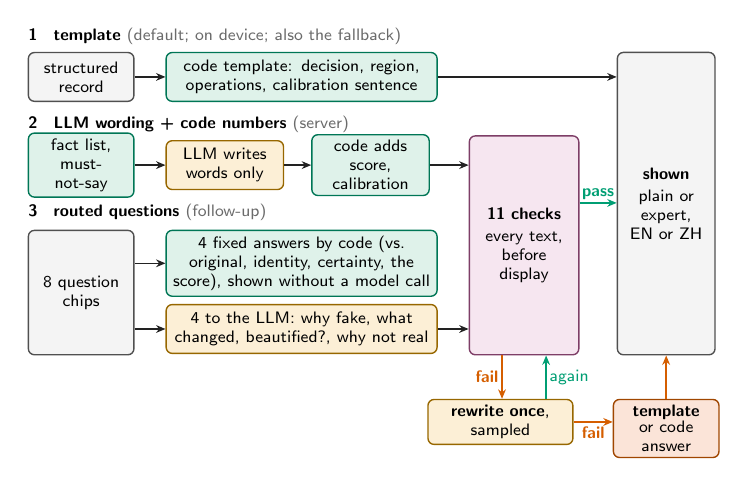
\begin{tikzpicture}[x=1cm,y=1cm]
\tier{0.52}{1}{template \textcolor{muted}{\textmd{(default; on device; also the fallback)}}}
\node[io, b, anchor=west, text width=1.2cm] (r1) at (0,0) {structured record};
\node[code, b, anchor=west, text width=3.3cm] (t1) at (1.75,0) {code template: decision, region, operations, calibration sentence};

\tier{-0.6}{2}{LLM wording + code numbers \textcolor{muted}{\textmd{(server)}}}
\node[code, b, anchor=west, text width=1.2cm] (f2) at (0,-1.12) {fact list, must-not-say};
\node[llm, b, anchor=west, text width=1.35cm] (l2) at (1.75,-1.12) {LLM writes words only};
\node[code, b, anchor=west, text width=1.35cm] (c2) at (3.6,-1.12) {code adds score, calibration};

\tier{-1.72}{3}{routed questions \textcolor{muted}{\textmd{(follow-up)}}}
\node[io, b, anchor=north west, text width=1.2cm, minimum height=1.58cm] (q3) at (0,-1.94) {8 question chips};
\node[code, b, anchor=north west, text width=3.3cm] (fx) at (1.75,-1.94) {4 fixed answers by code (vs.\ original, identity, certainty, the score), shown without a model call};
\node[llm, b, anchor=south west, text width=3.3cm] (lq) at (1.75,-3.52) {4 to the LLM: why fake, what changed, beautified?, why not real};

\node[chk, b, anchor=north west, text width=1.25cm, minimum height=2.78cm] (ck) at (5.6,-0.74) {\textbf{11 checks}\\[1pt]every text, before display};
\node[io, b, anchor=north west, text width=1.1cm, minimum height=3.84cm] (dp) at (7.48,0.32) {\textbf{shown}\\[1pt]plain or expert, EN or ZH};

\draw[flow] (r1) -- (t1);
\draw[flow] (t1.east) -- (dp.west |- t1.east);
\draw[flow] (f2) -- (l2); \draw[flow] (l2) -- (c2); \draw[flow] (c2.east) -- (ck.west |- c2.east);
\draw[flow] (q3.east |- fx.west) -- (fx.west); \draw[flow] (q3.east |- lq.west) -- (lq.west);
\draw[flow] (lq.east) -- (ck.west |- lq.east);
\draw[okflow] (ck.east |- 0,-1.6) -- node[above, font=\fontsize{5.6}{6}\selectfont\bfseries, text=okc, inner sep=1pt]{pass} (dp.west |- 0,-1.6);

\coordinate (ckS) at (ck.south);
\node[llm, b, anchor=north, text width=1.7cm, minimum height=0.5cm] (rw) at ([xshift=-0.3cm,yshift=-0.55cm]ckS) {\textbf{rewrite once}, sampled};
\node[fall, b, anchor=north, text width=1.2cm, minimum height=0.5cm] (tp) at (rw.north -| dp.south) {\textbf{template}\\[-1pt]or code answer};
\draw[errflow] ([xshift=-0.28cm]ckS) -- node[left, font=\fontsize{5.6}{6}\selectfont\bfseries, text=errc, inner sep=1pt]{fail} ([xshift=-0.28cm]ckS |- rw.north);
\draw[okflow] ([xshift=0.28cm]ckS |- rw.north) -- node[right, font=\fontsize{5.6}{6}\selectfont, text=okc, inner sep=1pt]{again} ([xshift=0.28cm]ckS);
\draw[errflow] (rw.east) -- node[below, font=\fontsize{5.6}{6}\selectfont\bfseries, text=errc, inner sep=1.5pt]{fail} (tp.west |- rw.east);
\draw[errflow] (tp.north) -- (dp.south);
\end{tikzpicture}
\end{document}
